\section{Evaluation}
\subsection{Experiments}

\begin{frame}{The Applicative \textbf{olac}}
	\begin{itemize}[<+-| alert@+>]
		\item In the applicative \textbf{olac} we have the implementation of three different approaches of an association rules based classifier:
		\begin{itemize}[<+-| alert@+>]
			\item The LAC (\textit{Lazy Associative Classifier}) approach, that is the \textit{lazy} strategy in his original version(and non-orthogonal);
			\item The OLAC (\textit{Orthogonal Lazy Associative Classifier}) approach, that is a variant of the \textit{lazy} strategy considering orthogonality;
			\item The ORIGAMI, that is the adaptation presented for the ORIGAMI strategy.
		\end{itemize}
	\end{itemize}
\end{frame}

%\begin{frame}[fragile,shrink=30]{Op��es de Execu��o}
%
%\begin{verbatim}
%Usage: ./olac [options]
%Options:
%  -i, --training-file       Set the training file
%  -t, --testing-file        Set the testing file
%  -s, --support             Set the support
%  -c, --confidence          Set the confidence
%  -r, --run-mode            Set the run mode [c,o] [CLASSICAL, ORTHOGONAL]
%  -p, --pattern-set         Set the pattern set type [f,m,r] [FREQUENT, MAXIMAL,
%                              RANDOM MAXIMAL]
%  -n, --min-num-rules       Set the minimum number of rules generated
%  -l, --max-num-rank-rules  Set the maximum number of rules considered (rank size)
%  -m, --min-rule-len        Set the minimum length of the rules
%  -x, --max-rule-len        Set the maximum length of the rules
%  -o, --orth-mode           Set the orthogonality mode [h,p,o] [HEURISTICAL,
%                              POLYNOMIAL, ORIGAMI]
%\end{verbatim}
%
%\end{frame}

%\begin{frame}[fragile,shrink=30]{Op��es de Execu��o}
%
%\begin{verbatim}
%  -e, --orth-metric         Set the orthogonality metric [s,c,l,a] [STRUCTURE,
%                              TRANSACTION COVERAGE, CLASS COVERAGE, ALL]
%  -w, --orth-method         Set the way metrics are used [s,p,a] [SET, PAIR AVERAGE,
%                              ALL]
%  -g, --orth-pat-ordering   Set the way patterns are ordered for heuristic
%                              [s,r,i,z,n] [SORTED, REVERSE SORTED, SORTED BY SIZE,
%                              REVERSE SORTED BY SIZE, NONE]
%  -u, --rule-measure        Set the rule measure used [s,c,j,k,o,n,e,p,l,i,v]
%                              [SUPPORT, CONFIDENCE, JACCARD, KULC, COSINE,
%                              CONVICTION, SENSITIVITY, SPECIFICITY, LAPLACE,
%                              LIFT, LEVERAGE]
%  -a, --origami-alpha       Set the alpha parameter used by ORIGAMI
%  -b, --origami-beta        Set the beta parameter used by ORIGAMI
%  -d, --debug               Set the level of debug [-1,0,1,2,3,4] [SILENT, NO DEBUG,
%                              LOW LEVEL, MEDIUM LEVL, HIGH LEVEL, MAX LEVEL]
%  -v, --verbose             Use verbose mode
%  -h, --help                Display this information
%\end{verbatim}
%
%\end{frame}

%\subsection{Experimentos}

\begin{frame}{Methodology}
	\begin{itemize}[<+-| alert@+>]
		\item We used 26 datasets from \textbf{UCI} (\textit{UC Irvine Machine Learning Repository});
		\item We used 10-fold cross-validation and the final results of each experiment represent the average of the ten runs.
			\end{itemize}
\end{frame}

%\begin{frame}{Metodologia}
%	\begin{itemize}[<+-| alert@+>]
%		\item Como resultados foram considerados a m�dia das dez execu��es diferentes para cada base de dados;
%		\item Os par�metros utilizados nos testes se encontram na tabela \ref{tab:table_test_parms_presentation};
%		\item Todas as combina��es poss�veis destes par�metros foram realizadas, com exce��o da combina��o tamanho m�ximo de regra  $1$ e m�trica de ortogonalidade $s$ para o OLAC.
%	\end{itemize}
%\end{frame}

\begin{frame}[shrink]{Methodology}
	\begin{centering}
	\begin{table}[htbp]
	\centering
		\resizebox{0.95\textwidth}{!} {
		\begin{tabular}{|l|c|}
		\hline
		\textbf{Parameters}	& \textbf{Values}	\\
		\hline
		support			& $\left\{ 0.0001, 0.001, 0.01, 0.1, 0.2, 0.3, 0.4, 0.5, 0.6, 0.7, 0.8, 0.9, 0.95, 0.99, 1 \right\}$	\\
		\hline
		confidence		& $\left\{ 0.0001, 0.001, 0.01, 0.1, 0.2, 0.3, 0.4, 0.5, 0.6, 0.7, 0.8, 0.9, 0.95, 0.99, 1 \right\}$				\\
		\hline
		min-num-rules		& $\left\{ 1 \right\}$				\\
		\hline
		max-num-rank-rules	& $\left\{ 1,10,100,1000,10000,100000,1000000 \right\}$		\\
		\hline
		min-rule-len		& $\left\{ 1 \right\}$				\\
		\hline
		max-rule-len		& $\left\{ 1,2,3 \right\}$		\\
		\hline
		rule-measure		& $\left\{ s,c,j,k,o,n,e,p,l,i,v \right\}$	\\
		\hline
		orth-metric		& $\left\{ e,c,l,a \right\}$			\\
		\hline
		orth-method		& $\left\{ s,p \right\}$				\\
		\hline
		orth-pat-ordering	& $\left\{ s,r,i,z,n \right\}$			\\
		\hline
		origami-alpha		& $\left\{ 0.1,0.2,0.3,0.4,0.5,0.6,0.7,0.8,0.9 \right\}$		\\
		\hline
		origami-beta		& $\left\{ 0.1,0.2,0.3,0.4,0.5,0.6,0.7,0.8,0.9 \right\}$		\\
		\hline
		\end{tabular}
		}
	\caption{Parameters Used for All Approaches}
	\label{tab:table_test_parms}
\end{table}

	\end{centering}
\end{frame}

\begin{frame}[shrink]{Better Results for Each Dataset}
	\begin{centering}
	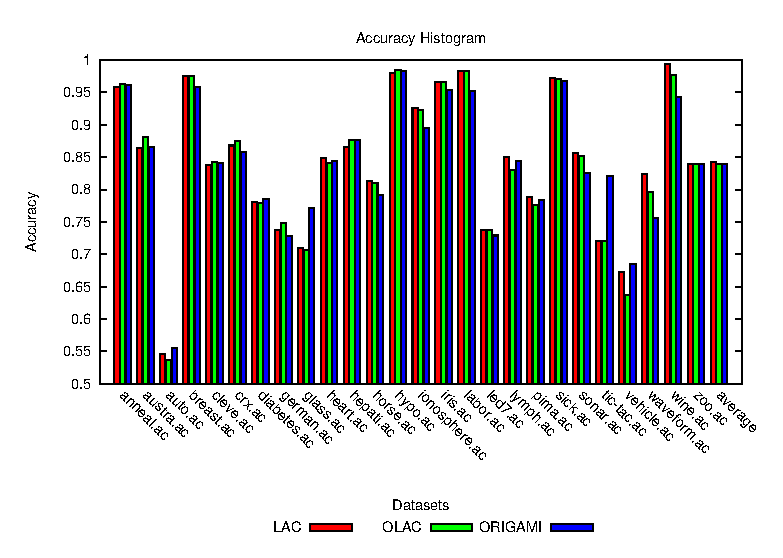
\includegraphics[width=\textwidth]{../thesis/graphs/histogram_best_run_for_each_db_acc_en}
	\end{centering}
\end{frame}

\begin{frame}[shrink]{Better Results for Each Dataset}
	\begin{centering}
	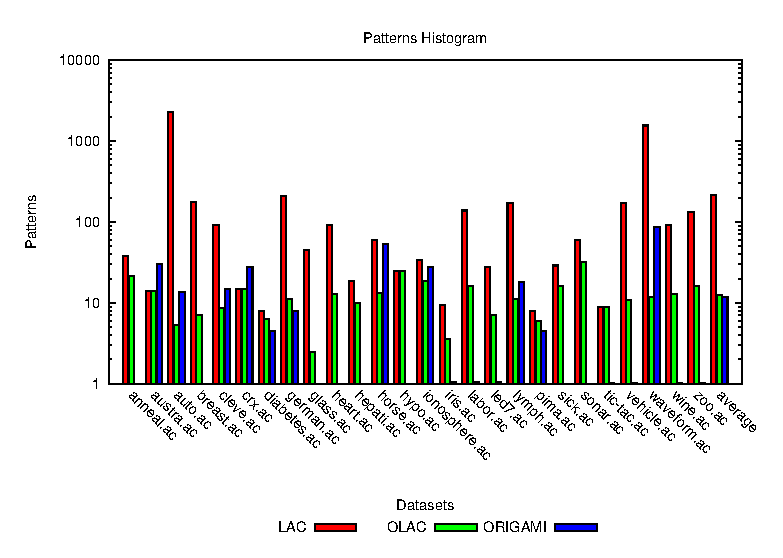
\includegraphics[width=\textwidth]{../thesis/graphs/histogram_best_run_for_each_db_pat_en}
	\end{centering}
\end{frame}

\begin{frame}[shrink]{Better Results for Each Dataset}
	\begin{centering}
	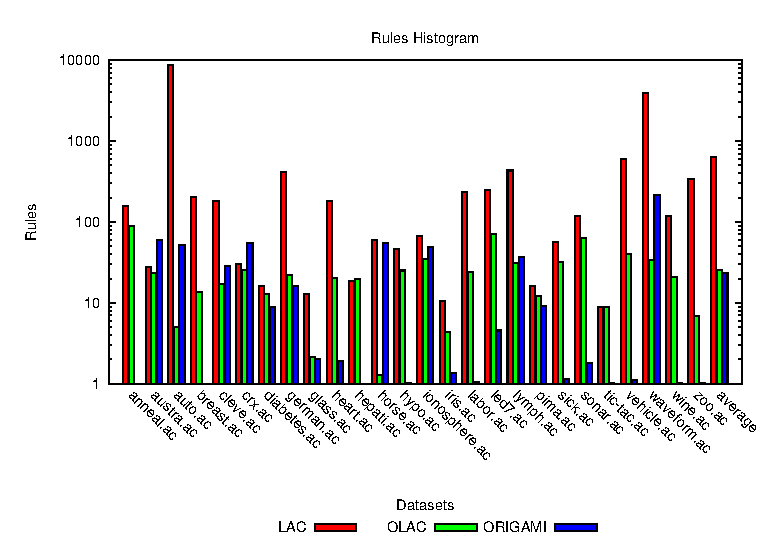
\includegraphics[width=\textwidth]{../thesis/graphs/histogram_best_run_for_each_db_rul_en}
	\end{centering}
\end{frame}

\begin{frame}[shrink]{Better Results in Average for All Datasets}
	\begin{centering}
	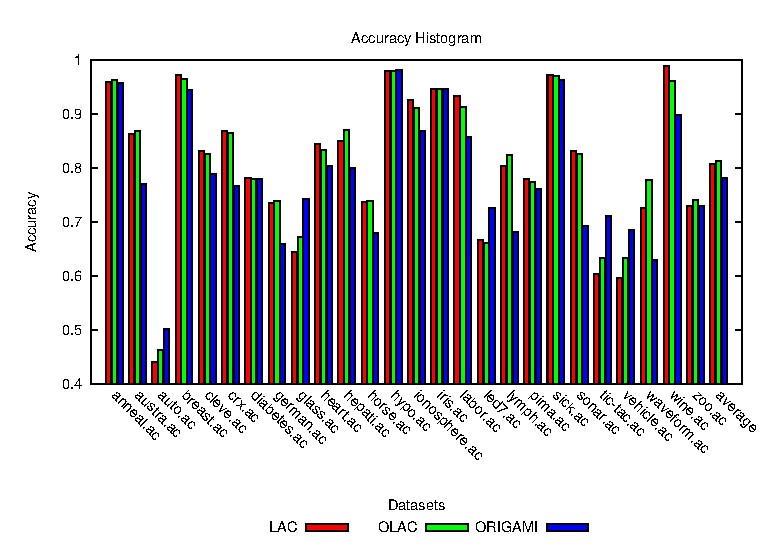
\includegraphics[width=\textwidth]{../thesis/graphs/histogram_best_run_for_avg_db_acc_en}
	\end{centering}
\end{frame}

\begin{frame}[shrink]{Better Results in Average for All Datasets}
	\begin{centering}
	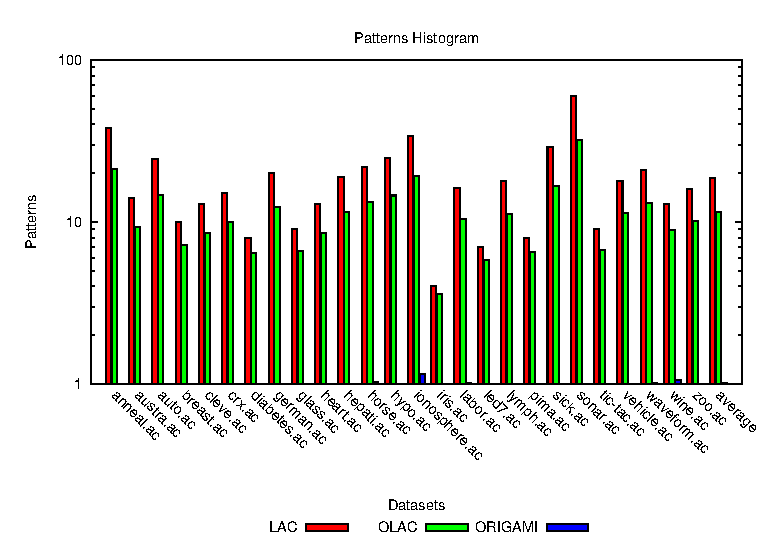
\includegraphics[width=\textwidth]{../thesis/graphs/histogram_best_run_for_avg_db_pat_en}
	\end{centering}
\end{frame}

\begin{frame}[shrink]{Better Results in Average for All Datasets}
	\begin{centering}
	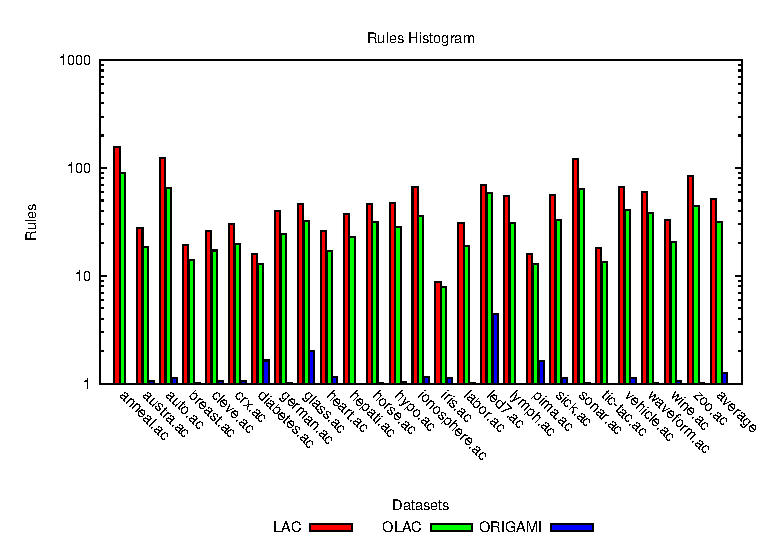
\includegraphics[width=\textwidth]{../thesis/graphs/histogram_best_run_for_avg_db_rul_en}
	\end{centering}
\end{frame}

\begin{frame}[shrink]{Execution Parameters}
	\begin{centering}
	\begin{table}[htbp]
	\centering
		\renewcommand{\tabcolsep}{1.8mm}
		\begin{tabular}{|l|c|c|c|}
		\hline
					& \textbf{LAC}	& \textbf{OLAC}	& \textbf{ORIGAMI}	\\
		\hline
		support			& 0.001	& 0.0001	& 0.0001		\\
		\hline
		confidence		& 0.01		& 0.0001	& 0.0001		\\
		\hline
		min-num-rules		& 1		& 1		& 1			\\
		\hline
		max-num-rank-rules	& 1000		& 100		& 10			\\
		\hline
		min-rule-len		& 1		& 1		& -			\\
		\hline
		max-rule-len		& 1		& 2		& -			\\
		\hline
		rule-measure		& n		& n		& c			\\
		\hline
		orth-metric		& -		& s		& s			\\
		\hline
		orth-method		& -		& s		& -			\\
		\hline
		orth-pat-ordering	& -		& s		& -			\\
		\hline
		origami-alpha		& -		& -		& 0.1			\\
		\hline
		origami-beta		& -		& -		& 0.8			\\
		\hline
		\end{tabular}
	\caption{Best Parameters for Each Run}
	\label{tab:best_parms_for_avg_db}
\end{table}
	\end{centering}
\end{frame}

\begin{frame}
	\begin{block}{Results obtained with LAC using the best parameters for OLAC}
		Patterns: $249.03$ \\
		Rules: $628.12$ \\
		Accuracy: $0.54$
	\end{block}
\end{frame}

\begin{frame}[shrink]{Comparing the Results}
	\begin{centering}
	\begin{table}[htbp]
	\centering
%		\resizebox{0.95\textwidth}{!} {
		\begin{tabular}{|l|c|c|c|c|}
		\hline
				& \textbf{OLAC}		& \textbf{OLAC}			& \textbf{$\neg$ OLAC}	& \textbf{$\neg$ OLAC}	\\
		\textbf{Datasets}	& \textbf{\&}		& \textbf{\&}			& \textbf{\&}			& \textbf{\&}			\\
				& \textbf{LAC}		& \textbf{$\neg$ LAC}		& \textbf{LAC}			& \textbf{$\neg$ LAC}		\\
		\hline
		anneal.ac       & 95.11         & 1.13               & 0.75                     & 3.01                          \\
		\hline
		austra.ac       & 84.93         & 1.88               & 1.45                     & 11.74                         \\
		\hline
		auto.ac         & 39.51         & 6.83               & 4.39                     & 49.27                         \\
		\hline
		breast.ac       & 96.28         & 0.29               & 1.00                     & 2.43                          \\
		\hline
		cleve.ac        & 81.19         & 1.32               & 1.98                     & 15.51                         \\
		\hline
		crx.ac          & 84.93         & 1.59               & 1.88                     & 11.59                         \\
		\hline
%		diabetes.ac     & 76.82         & 1.04               & 1.30                     & 20.83                         \\
%		\hline
%		german.ac       & 70.40         & 3.40               & 3.10                     & 23.10                         \\
%		\hline
%		glass.ac        & 63.08         & 4.21               & 1.40                     & 31.31                         \\
%		\hline
%		heart.ac        & 82.96         & 0.37               & 1.48                     & 15.19                         \\
%		\hline
%		hepati.ac       & 85.16         & 1.94               & 0.00                     & 12.90                         \\
%		\hline
%		horse.ac        & 70.38         & 3.53               & 3.26                     & 22.83                         \\
%		\hline
%		hypo.ac         & 97.94         & 0.06               & 0.09                     & 1.90                          \\
%		\hline
%		ionosphere.ac   & 90.03         & 1.14               & 2.56                     & 6.27                          \\
%		\hline
%		iris.ac         & 94.00         & 0.67               & 0.67                     & 4.67                          \\
%		\hline
%		labor.ac        & 89.47         & 1.75               & 3.51                     & 5.26                          \\
%		\hline
%		led7.ac         & 61.72         & 4.31               & 4.97                     & 29.00                         \\
%		\hline
%		lymph.ac        & 79.73         & 2.70               & 0.68                     & 16.89                         \\
%		\hline
%		pima.ac         & 76.82         & 0.52               & 1.04                     & 21.61                         \\
%		\hline
%		sick.ac         & 97.04         & 0.04               & 0.18                     & 2.75                          \\
%		\hline
%		sonar.ac        & 80.29         & 2.40               & 2.88                     & 14.42                         \\
%		\hline
%		tic-tac.ac      & 56.47         & 6.78               & 3.86                     & 32.88                         \\
%		\hline
%		vehicle.ac      & 56.86         & 6.50               & 2.72                     & 33.92                         \\
%		\hline
%		waveform.ac     & 71.12         & 6.74               & 1.54                     & 20.60                         \\
%		\hline
		$\vdots$        & $\vdots$      & $\vdots$           & $\vdots$                 & $\vdots$                      \\
		\hline
		wine.ac         & 96.07         & 0.00               & 2.81                     & 1.12                          \\
		\hline
		zoo.ac          & 73.27         & 0.99               & 0.00                     & 25.74                         \\
		\hline
		average         & 78.91         & 2.39               & 1.90                     & 16.80                         \\
		\hline
		\end{tabular}
%		}
	\caption{Comparison between LAC and OLAC (number of correct and wrong classifications)}
	\label{tab:comparison_lac_olac}
\end{table}

	\end{centering}
\end{frame}

% O Aplicativo olac
% Exemplo de Execu��o
% Experimentos
